%!TEX root = ../Diploma.tex


\begin{section}{Проведенные эксперименты}

Для обучения было использовано 40\% начальной выборки. В процессе оптимизации гиперпараметров для каждого классификатора использовалась кросс-валидация (CV-10). Кросс-валидация способствует минимизации риска  переобучения, и следовательно,  смещения в оценке качества классификатора. Оптимизация проводилась для обоих групп признаков (каждый признак был нормализован и принимал значение в диапазоне [-1, 1]). Кроме этого для настройки SVM было отобрано 30\% наиболее значимых признаков по критерию хи-квадрат, поскольку это более оптимально с точки зрения вычислительной нагрузки.

Далее приведены результаты оптимизации гиперпараметров с помощью полного перебора по сетке.

\begin{subsection}{Подбор параметров по сетке}

\begin{subsubsection}{Naive Bayes}
Единственным параметром, по которому проходил поиск по сетке для наивного байесовского классификатора, это параметр \textit{fit\_prior}, который принимает булевые значения \textit{True} или \textit{False}. Суть этого параметра в использовании предыдущих вероятностей класса при обучении или их игнорировании.

\begin{table}[H]
\centering
{\begin{tabular}{|l|c|c|}
\hline
\textbf{Fit\_Prior} & \textbf{Accuracy} & \textbf{Std} \\
\hline
True & 0.75619  & 0.00392 \\
\hline
\textbf{False} & \textbf{0.75718}  & \textbf{0.8549} \\
\hline
\end{tabular}}

\caption{Подбор по сетке Naive Bayes}
\label{grid:nb}
\end{table}



\end{subsubsection}



\begin{subsubsection}{\textit{k}-nearest neighbors}
  Для алгоритма \textit{k}-NN оптимальной оказалась модель с \textit{k} = 13 и применением весов, зависящих от расстояния до соседа (см. п. \ref{alg:knn})

  \begin{table}[H]
  \centering
  {\begin{tabular}{|l|l|c|c|}
  \hline
  \textbf{Number of neighbors \textit{k}} & \textbf{Weights} & \textbf{Accuracy} & \textbf{Std} \\
  \hline
  k = 1 & uniform  & 0.8549 & 0.00398 \\
  \hline
  k = 1 & distance  & 0.8549 & 0.00398 \\
  \hline
  k = 3 & uniform  & 0.87634 & 0.00353 \\
  \hline
  k = 3 &  distance & 0.87596  & 0.00346 \\
  \hline
  k = 5 & uniform  & 0.88281 & 0.00304 \\
  \hline
  k = 5 & distance  & 0.88302 & 0.00295 \\
  \hline
  k = 7 & uniform  & 0.88481 & 0.00367 \\
  \hline
  k = 7 &  distance & 0.88525  & 0.00360 \\
  \hline
  k = 9 & uniform  & 0.88546 & 0.00424 \\
  \hline
  k = 9 & distance  & 0.88635 & 0.00401 \\
  \hline
  k = 11 & uniform  & 0.88560 & 0.00432 \\
  \hline
  k = 11 &  distance & 0.88737  & 0.00448 \\
  \hline
  k = 13 & uniform  & 0.88618 &  0.00394 \\
  \hline
  \textbf{k = 13} & \textbf{distance}  & \textbf{0.88844} & \textbf{0.00369} \\
  \hline
  k = 15 & uniform  & 0.88612 & 0.00359 \\
  \hline
  k = 15 &  distance & 0.88802  & 0.00272 \\
  \hline
  k = 17 & uniform  & 0.88551 & 0.00345 \\
  \hline
  k = 17 & distance  & 0.88797 & 0.00300 \\
  \hline
  k = 19 & uniform  & 0.88481 & 0.00315 \\
  \hline
  k = 19 &  distance & 0.88802  & 0.00361 \\
  \hline
  \end{tabular}}

  \caption{Подбор по сетке \textit{k}-NN}
  \label{grid:knn}
  \end{table}



\end{subsubsection}

\begin{subsubsection}{SVM}

Для алгоритма SVM оптимальной оказалась модель с сигмоидом в качестве ядра (см. пункт \ref{svm})
  \begin{table}[H]
  \centering
  {\begin{tabular}{|l|c|c|}
  \hline
  \textbf{Kernel} & \textbf{Accuracy} & \textbf{Std} \\
  \hline
  linear & 0.88560 & 0.00432 \\
  \hline
  poly & 0.88481 & 0.00401 \\
  \hline
  rbf & 0.8549 & 0.00394 \\
  \hline
  \textbf{sigmoid} & \textbf{0.88802} & \textbf{0.00398} \\
  \hline
  precomputed & 0.8549 & 0.00300 \\
  \hline
  \end{tabular}}

  \caption{Подбор по сетке \textit{k}-NN}
  \label{grid:svm}
  \end{table}

\end{subsubsection}

\begin{subsubsection}{Decision tree}

Для алгоритма Decision tree оптимальной оказалась модель с использованием меры энтропии в качестве критерия расщепления (см. пункт \ref{dt}), без использования ограничений на глубину дерева, а также стратегией расщепления нацеленной на <<наилучшее>>, а не случайное расщепление.


\begin{table}[H]
\centering
{\begin{tabular}{|l|l|l|c|c|}
\hline
\textbf{Criterion} & \textbf{Max depth} & \textbf{Splitter} & \textbf{Accuracy} & \textbf{Std} \\
\hline
Gini & 1  & best & 0.84177 & 0.00516 \\
\hline
Gini & 1  & random &  0.54702 & 0.03000 \\
\hline
Gini & 2  & best & 0.84177 & 0.00516 \\
\hline
Gini &  2 & random  & 0.59500 & 0.02743 \\
\hline
Gini & 3  & best & 0.87258 & 0.00449 \\
\hline
Gini & 3  & random & 0.64052 & 0.07874 \\
\hline
Gini & None  & best & 0.88475 & 0.00386 \\
\hline
Gini &  None & random  & 0.87360 & 0.00496 \\
\hline
Entropy & 1  & best & 0.84182 & 0.00480 \\
\hline
Entropy & 1  & random & 0.55109 & 0.03190 \\
\hline
Entropy  & 2  & best & 0.84182 & 0.00480 \\
\hline
Entropy  &  2 & random  & 0.58652 & 0.03546 \\
\hline
Entropy  & 3  & best &  0.86879 & 0.00419 \\
\hline
Entropy  & 3  & random & 0.67764 & 0.06590 \\
\hline
\textbf{Entropy} & \textbf{None}  & \textbf{best} & \textbf{0.88884} & \textbf{0.00441} \\
\hline
Entropy &  None & random  & 0.87409 & 0.00369 \\
\hline
\end{tabular}}

\caption{Подбор по сетке DT}
\label{grid:dt}
\end{table}


\end{subsubsection}


\begin{subsubsection}{Random forest}

Для алгоритма Random forest оптимальной оказалась модель, состоящая из 19 деревьев, с использованием меры энтропии в качестве критерия расщепления (см. пункт \ref{dt}), без использования ограничений на глубину деревьев и без использования бутстрапа (см. пункт \ref{rf}).

  \begin{table}[H]
  \centering
  {\begin{tabular}{|l|l|l|l|c|c|}
  \hline
  \textbf{Estimators} & \textbf{Criterion} & \textbf{Max Depth} & \textbf{Bootstrap} & \textbf{Accuracy} & \textbf{Std} \\
  \hline
  1 & entropy  & None & False & 0.88533 & 0.00387 \\
  \hline
  2 & entropy  & None &  False & 0.87751 & 0.00397 \\
  \hline
  3 & entropy  & None & False & 0.91223 & 0.00430 \\
  \hline
  4 &  entropy & None  & False & 0.90904 & 0.00313 \\
  \hline
  5 & entropy  & None & False & 0.91826 & 0.00300 \\
  \hline
  6 & entropy  & None & False & 0.91656 & 0.00358 \\
  \hline
  7 & entropy  & None & False & 0.92170 & 0.00378 \\
  \hline
  8 &  entropy & None  & False & 0.92052 & 0.00251 \\
  \hline
  9 & entropy  & None & False & 0.92294 & 0.00340 \\
  \hline
  10 & entropy  & None & False & 0.92216 & 0.00363 \\
  \hline
  11  & entropy  & None & False & 0.92441 & 0.00347 \\
  \hline
  12  &  entropy & None  & False & 0.92423 & 0.00263 \\
  \hline
  13  & entropy  & None &  False & 0.92441 & 0.00258 \\
  \hline
  14  & entropy  & None & False & 0.92523 & 0.00323 \\
  \hline
  15 & entropy  & None & False & 0.92617 & 0.00309 \\
  \hline
  16 &  entropy & None  & False & 0.92571 & 0.00254 \\
  \hline
  17 & entropy  & None & False & 0.92643 & 0.00405 \\
  \hline
  18 & entropy  & None &  False & 0.92645 & 0.00305 \\
  \hline
  \textbf{19} & \textbf{entropy}  & \textbf{None} & \textbf{False} & \textbf{0.92685} & \textbf{0.00312} \\
  \hline
  \end{tabular}}

  \caption{Подбор по сетке Random Forest}
  \label{grid:rf}
  \end{table}



\end{subsubsection}

\end{subsection}

\begin{subsection}{Выбор классификатора}

  После оптимизации гиперпараметров каждый из алгоритмов оценивался на оставшихся 60\% данных с использованием обоих групп признаков и CV-10. Также как и в случае поиска по сетке, каждый признак был нормализован, а для SVM использовалось 30\% наиболее значимых признаков по критерию хи-квадрат.


В качестве метрик оценки классификаторов были выбраны полнота (R), точность (P) и F-мера. Метрика полноты представляет из себя отношение числа сообщений, корректно классифицированных как спам (True Positives) и общего числа спамовых сообщений (True Positives + False Negatives):

\begin{equation}
  R = \frac{True Positives}{True Positives + False Negatives}
\end{equation}

Точность - это отношение числа сообщений, корректно классифицированных как спам (True Positives) и общего числа  сообщений, классифицированных как спам (True Positives + False Positives):

\begin{equation}
  P = \frac{True Positives}{True Positives + False Positives}
\end{equation}

F-мера может быть проинтерпретирована как гармоническое среднее между метриками точности и полноты:

\begin{equation}
  F1 = \frac{2 \times P \times R}{P + R}
\end{equation}

Как видно из таблицы \ref{tab:results}, классификаторы на основе дерева показали лучший результат. Random Forests обошел остальные классификаторы по показателю F-меры. Наилучший известный мне результат в данной задаче был достигнут у Lee \cite{Lee} и составляет 98\% по той же оценке F-меры. Однако Lee использовал историчные признаки, что является ограничением в нашем случае, следовательно, результат можно считать вполне неплохим. Это говорит о том, что лишь те признаки, которые можно извлечь непосредственно из твита и его метаданных,  могут служить хорошей основой для классификатора.


\begin{table}[H]
\centering
{\begin{tabular}{|l|c|c|c|}
\hline
\textbf{Классификатор} & \textbf{Точность} & \textbf{Полнота} & \textbf{F-мера}  \\
\hline
Naive Bayes & 76\% & 76\% & 76\% \\
\hline
\textit{k}-NN & 86\% & 86\% & 86\% \\
\hline
SVM & 86\% & 86\% & 86\%  \\
\hline
Decision Tree & 89\% & 89\% & 89\% \\
\hline
\textbf{Random Forest} & \textbf{93\%} & \textbf{93\%} & \textbf{93\%} \\
\hline
\end{tabular}}
\caption{Сравнение показателей классификаторов}
\label{tab:results}
\end{table}



\end{subsection}


\begin{subsection}{Оценка признаков}
Для оценки значимости признаков были использованы их различные комбинации  при обучении классификаторов. Результат однозначно показал, что наибольший вес с точки зрения F-меры имеют признаки из пользовательской группы. Комбинации с использованием признаков из этой группы с различными признаками из группы признаков контента дают лишь небольшой прирост в F-мере.

Еще одним важным аспектом, который желательно учитывать при отборе признаков, это время их вычисления, особенно если существует необходимость применения классификатора в режиме реального времени. Таблица \ref{tab:comptime} демонстрирует время вычисления каждой из групп признаков для 1000 твитов со следующими параметрами машины:
\begin{enumerate}
\item CPU: Intel Core i7
\item RAM: 16GB
\item OS: Ubuntu 16.04 64-bit
\end{enumerate}



\begin{table}[H]
\centering
\resizebox{\textwidth}{!}{\begin{tabular}{|l|c|}
\hline
\textbf{Группа признаков} & \textbf{Время на вычисление (сек.) для 1000 твитов} \\
\hline
Пользовательские признаки & 0.0057 \\
\hline
Признаки контента & 1.0448 \\
\hline
\end{tabular}}

\caption{Время вычисления признаков}
\label{tab:comptime}
\end{table}

Следует отметить, что обе группы признаков вычисляются за приемлемое время, что отвечает условиям поставленной задачи, однако такие признаки как \textit{Количество спамовых слов (КСП)} и \textit{Количество спамовых слов на одно слово (КСП/КС)}
\end{subsection} наиболее затратны с точки зрения вычисления и не приносят ощутимого прироста в точность модели, что можно предположительно можно обьяснить тем, что большинство из этих спамовых слов взяты из рекламных блогов и спамовых писем, для которых нехарактерна спамовая семантика коротких сообщений, поэтому этот признак можно исключить из выборки из соображений эффективности времени работы классификатора.


\begin{subsection}{Анализ результатов}
Наиболее качественный результат был получен с помощью алгоритма Random Forest. Из всех признаков наиболее весомыми с точки зрения точности классификатора показали себя пользовательские признаки, такие как: \textit{Прирост Подписок, Количество Подписок, Репутация} и т.д. (см рис. \ref{pic:feature_importance})

\begin{figure}[ht!]
\centering
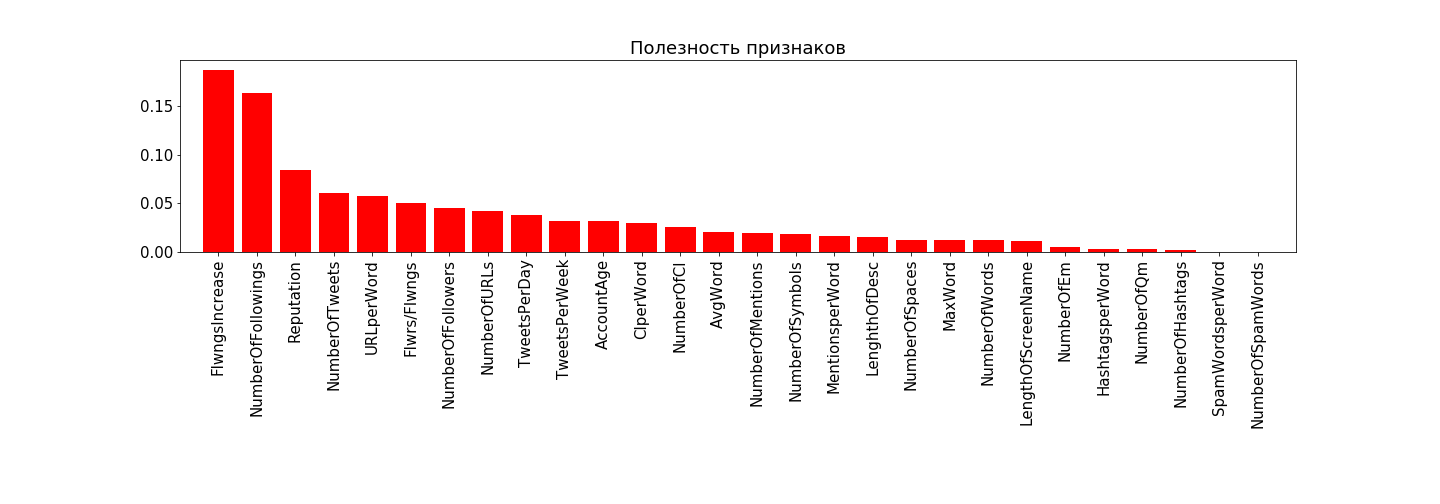
\includegraphics[width=1.0\textwidth]{pics/featureImportance.png}
\caption{Полезность признаков в алгоритме Random Forest}
\label{pic:feature_importance}
\end{figure}

Действительно, показатель \textit{Прирост Подписок} сильно отличается у спамовых и легитимных аккаунтов (см. рис. \ref{pic:flwngsincrease}). Это можно обьяснить тем, что спамовые аккаунты нацелены на охват максимально большой аудитории жертв за короткий промежуток времени.


\begin{figure}[ht!]
\centering
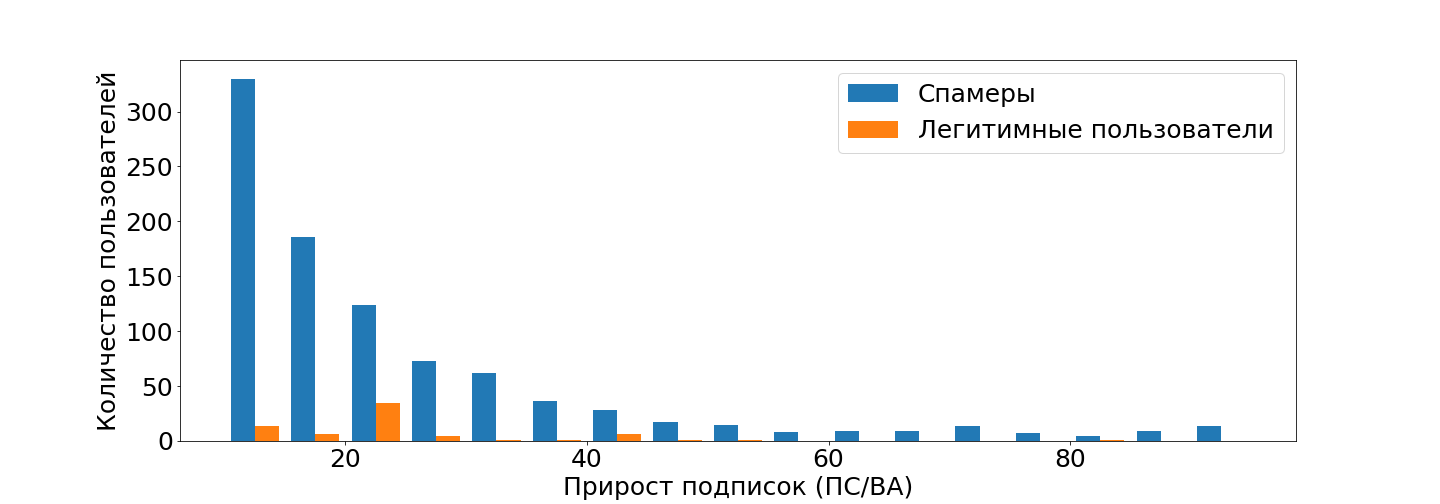
\includegraphics[width=1.0\textwidth]{pics/flwngsincrease.png}
\caption{Распределение пользователей по приросту подписок}
\label{pic:flwngsincrease}
\end{figure}

Кроме этого, на рисунке \ref{pic:ageincrease} можно наблюдать определенную положительную корреляцию между количеством подписок и возрастом аккаунта у спамовых пользователей. У легитимных аккаунтов подобная зависимость отсутствует.

\begin{figure}[ht!]
\centering
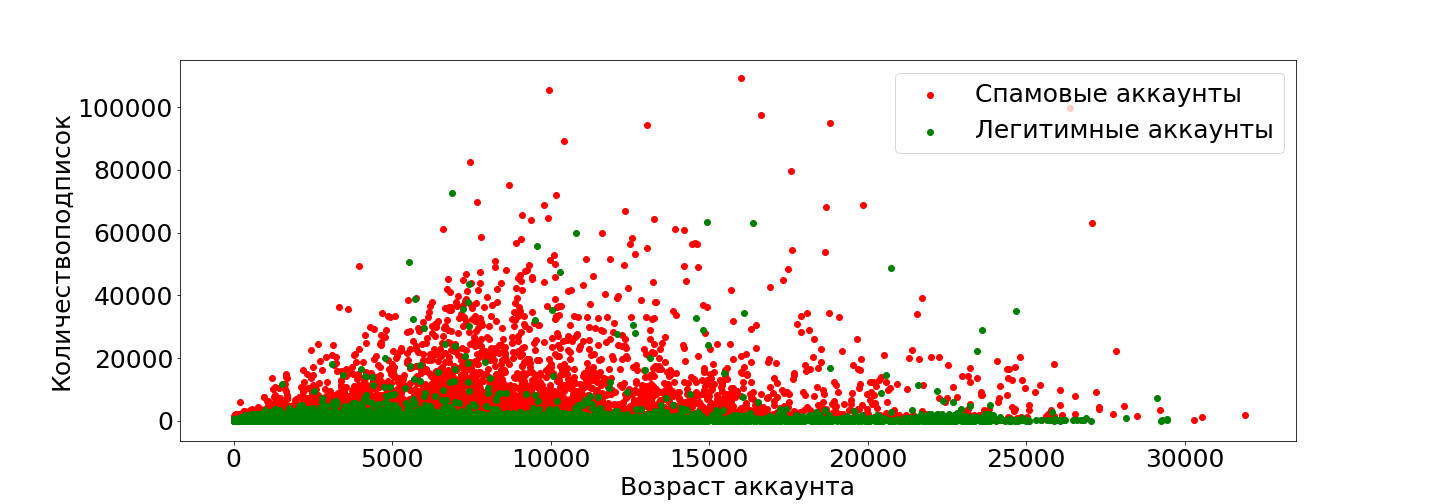
\includegraphics[width=1.0\textwidth]{pics/ageincrease.png}
\caption{Зависимость количества подписок от возраста аккаунта}
\label{pic:ageincrease}
\end{figure}


Посмотрим внимательнее на каких обьектах ошибается наш классификатор.

\begin{figure}[ht!]
\centering
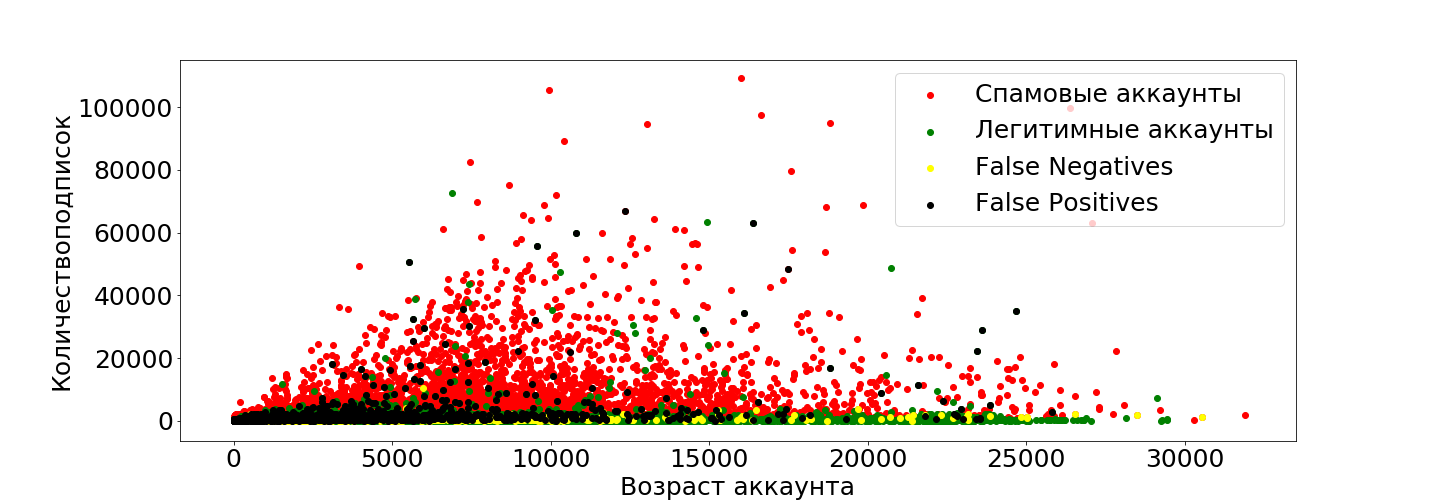
\includegraphics[width=1.0\textwidth]{pics/ageincreasewitherrors.png}
\caption{Зависимость количества подписок от возраста аккаунта}
\label{pic:ageincreasewithwerrors}
\end{figure}

Рисунок \ref{pic:ageincreasewithwerrors} позволяет убедится, что подавляющая доля ошибок происходит на пересечении классов.

Более чем в половине твитов, ошибочно классифицированных как спам, присутствуют ссылки (см. таблицу \ref{tab:urls}).



\begin{table}[H]
\centering
{\begin{tabular}{|l|c|}
\hline
\textbf{Количество ссылок} & \textbf{Доля в множестве FalsePositives} \\
\hline
0 &   39.565628 \\
\hline
1  &  58.545798 \\
\hline
2  &   1.416431 \\
\hline
5  &  0.094429 \\
\hline
\end{tabular}}

\caption{Наличие ссылок в ошибках}
\label{tab:urls}
\end{table}

Примеры неверно классифицированных твитов приведены в таблицах \ref{tab:fp} и \ref{tab:fp2}.


\begin{table}[H]
\centering
\resizebox{\textwidth}{!}{\begin{tabular}{|l|l|}
\hline
 \textbf{\#} & \textbf{Твит} \\
\hline
1 & If you aren't at SES Berlin, go to SES Chicago for 11 topics breaking http://tinyurl.com/yazwgcj \\
\hline
2 & Hummingbird 2, by far the best marketing tool for twitter. More Info! http://bit.ly/2K5Zon \\
\hline
3 & Need A Job? Hiring Today - Job Requires: Basic Computer Skills Your Own Home Computer. Weekly Pay : http://tinyurl.com/yzqyqoc \\
\hline
4 & Need Parking at any UK Airport? We have used and recommend these guys: http://tinyurl.com/r6a6tm Secure, convenient and affordable. \\
\hline
5 & We are recommending Essential Travel for affordable travel insurance throughout Europe from the UK: http://tinyurl.com/ozsjbw \\
\hline
\end{tabular}}

\caption{Примеры FalsePositives}
\label{tab:fp}
\end{table}




\begin{table}[H]
\centering
\resizebox{\textwidth}{!}{\begin{tabular}{|l|c|c|c|c|c|}
\hline
  \textbf{\#} &  \textbf{Количество Подписок} &  \textbf{Количество подписчиков} &  \textbf{Репутация} &  \textbf{Прирост подписок} &  \textbf{Твитов в день} \\
\hline
 1 &              1796.0 &             1040.0 &    0.366714 &        2.017978 &      2.453933 \\
\hline
 2 &              2807.0 &             2562.0 &    0.477184 &        0.976348 &      8.406261 \\
\hline
 3 &             17582.0 &            20181.0 &    0.534412 &        3.153156 &     13.635581 \\
\hline
 4 &             32596.0 &            30935.0 &    0.486928 &        5.770225 &     92.299522 \\
\hline
 5   &             35067.0 &            35122.0 &    0.500392 &        1.420867 &     23.990276 \\
\hline
\end{tabular}}

\caption{Примеры FalsePositives}
\label{tab:fp2}
\end{table}


Можно сделать вывод о том, что данные обьекты действительно очень похожи на спамовые, однако, в рамках политики пользования Twitter, они таковыми не являются.

Очевидно, что большую часть спама можно определить по пользовательским признакам (см. рис. \ref{pic:feature_importance}), однако полное игнорирование признаков контента при классификации спама не является разумным решением, поскольку их использование дает определенный прирост в точности. Кроме того, использование признаков контента усложняет задачу имитации благонадежности для спамовых аккаунтов. К примеру, спамер может купить себе подписчиков, чтобы казаться более легитимным, но в его сообщениях все равно останется <<спамовость>>, которая будет определена с помощью признаков контента.

Наиболее высокий известный мне результат в задаче классификации социального спама был достигнут Ли \cite{Lee} и составляет $98\%$ . В своей работе он протестировал 30 алгоритмов классификации, включая Naive Bayes, Logistic regression, SVM, Random Forest. Алгоритмы оценивались с помощью метрик полноты, точности и F-меры, а также кривой ошибок (ROC).  Помимо взятых мною признаков в данной работе использовались историчные признаки, такие как: \textit{Среднее количество ссылок (упоминаний, хештэгов) в твите},  \textit{Среднее количество  уникальных ссылок (упоминаний, хештэгов) в твите}, \textit{Средняя схожесть контента твитов пользователя}, \textit{Степень сжатия опубликованных твитов}. Наиболее высокая точность была продемонстрирована с использованием алгоритма Random Forest с применением бустинга - $98$\%.

Сантош помимо довольно распространенных алгоритмов машинного обучения (Байесовская сеть, SVM, Random Forest, \textit{k}-nn и т.д.) использовал классификаторы на основе сжатия текста (Динамические марковские цепи, Алгоритм сжатия PPM). Лучший результат также был получен с применением Random Forest - $96\%$ \cite{Santos}.

Другой нестандартный метод классификации социального спама -  алгоритм CIA \cite{Chao} - не показал высоких результатов, и посему позиционируется лишь как дополнение к другим методам классификации.

Можно сделать вывод, что Random Forest является оптимальным выбором в вопросе определения классификатора социального спама.

\end{subsection}









\end{section}
